\documentclass[11pt,letterpaper]{article}
\usepackage{amsmath}
\usepackage{amsxtra}
\usepackage{amstext}
\usepackage{amssymb}
\usepackage{latexsym}
\usepackage{dsfont} % for \mathds{N}
\usepackage{graphicx}
\usepackage{subfigure}
\usepackage{setspace}
\usepackage[margin=3cm]{geometry}
\usepackage{natbib}
\usepackage{lscape}
\usepackage{multirow}
\usepackage{longtable}
\usepackage{rotating}
\usepackage{authblk}
\usepackage{bbm}
\usepackage{verbatim}
\usepackage{url}
\usepackage{fullpage}
\usepackage{enumerate}

\setlength{\LTcapwidth}{6in}
\newenvironment{changemargin}[3]{%
  \begin{list}{}{%
    \setlength{\topsep}{0pt}%
    \setlength{\leftmargin}{#1}%
    \setlength{\rightmargin}{#2}%
    \setlength{\topmargin}{#3}%
    \setlength{\listparindent}{\parindent}%
    \setlength{\itemindent}{\parindent}%
    \setlength{\parsep}{\parskip}%
  }%
  \item[]}{\end{list}}
\DeclareMathAlphabet{\mathpzc}{OT1}{pzc}{m}{it}
\newtheorem{assumption}{Assumption}
\newcommand{\argmax}{\operatornamewithlimits{argmax}}
\newcommand{\argmin}{\operatornamewithlimits{argmin}}
\newcounter{subtables}

\makeatletter
\setlength{\abovecaptionskip}{6pt}   % 0.5cm as an example
\setlength{\belowcaptionskip}{6pt}   % 0.5cm as an example
\makeatother


\providecommand{\e}[1]{\ensuremath{\times 10^{#1}}}



\title{Problem Set 3: Structural Discrete Choice Models}
\author{Chris Conlon }
\begin{document}
\date{due: July 10}
\maketitle

\textit{Okay this one is tricky -- you are welcome to work in pairs-- you can submit in pairs as long as you promise to both contribute something}

\section*{Rust: The Stata Estimator (though a bit easier in R/Matlab)}
This is taken from Han Hong's problem set at Stanford, the idea is that we can use the arguments in Hotz-Miller (1993), or Pesendorfer Schmidt-Dengler (2008) to construct an optimization free method to recover the utility parameters in the Rust problem.\\

We began by defining the choice specific value function with $\epsilon_{it}$ i.i.d. and EV.
\begin{eqnarray*}
v(x,d) &=& u(x,d) + \beta \int \log \left ( \sum_{d' \in D} \exp ( v (x',d'))  \right) p(x' | x, d) dx' \\
v(x,d) &=& u(x,d) + \beta \int \log \left ( \sum_{d' \in D} \exp ( v (x',d') - v(x',1) )  \right) p(x' | x, d) dx'  + \beta \int v(x,1) p (x' | x,1) dx'\\
\end{eqnarray*}
\begin{enumerate}
\item Estimate $p(x' | x,d)$ non parametrically or parametrically (for example as a set of  multinomial with $n$ outcomes or an exponential distribution).  Call your estimate $\hat{p}(x' | x,d)$.
\item Estimate $p(d | x)$ (the CCP) non-parametrically. You can use the binomial logit model with a basis function (increasing number of terms) or you can use a kernel such as $\mathbf{ksdensity}$ or $\mathbf{ecdf}$.
\item Now use the Hotz-Miller inversion to estimate:  $\hat{v}(x,d) - \hat{v}(x,1) = \log \hat{p}(d|x) - \log \hat{p}(1|x)$
\item Normalize $u(x,1) = 0$ and so for $=1$  we have that 
\begin{eqnarray*}
v(x,1) &=& \beta \int v(x',1) p(x' | x,1) dx' + \beta \int \log \left( \sum_{d' \in D} \exp(\hat{v}(x',d') - \hat{v}(x',1)) \right) \hat{p}(x' | x,1) dx' \\
&=& \beta \int v(x',1) p(x' | x,1) dx' - \beta \int \log \left(\hat{p}(1| x') \right)  \hat{p}(x' | x,1) dx' \\
\end{eqnarray*}
This defines a fixed point that we can iterate on to obtain a nonparametric estimate of $\hat{v}(x,1)$.  Add this to $\hat{v}(x,d) - \hat{v}(x,1)$ to recover the choice specific value functions for $d=1,\ldots,D$.
\item  Once we know $\hat{v}(x,d)$ for all $d \in D$ we can recover the nonparametric estimate of $u(x,d)$ for $d \geq 2$ by 
\begin{eqnarray*}
\hat{u}(x,d) = \hat{v}(x,d) - \beta \int \log \left(\exp(\hat{v}(x',d') \right) \hat{p}(x' | x,d) dx'
\end{eqnarray*}
\end{enumerate}
This estimator should be very simple to implement (and only requires one fixed point) so we could do inference via the bootstrap if we wanted to.

\section*{BLP Demand Estimation}
This problem set uses data on ``Over the counter'' Headache medicine (i.e.
aspirin, tylenol and such) and was graciously provided by Vishal Singh, so if
you want good demand data make friends with Marketing people!\footnote{But I stole this from Alan Collard-Wexler!}The data is at the store/week level for 3 brands and 3 package sizes.
\begin{itemize}
\item Count: Number of People that go into the store each week. 
\item Promotion: Is there a promotion on the product that week. 
\item Price: Price of the package.
\item Week and Store are the time and market indicator.
\end{itemize}

Demographic data for this problem set is composed of the following:
\begin{itemize}
\item Income: Average income for area served by a particular store.
\item This varies with stores but not across weeks.
\end{itemize}

Assume a utility specification for $u_{ij}$, household $i$'s utility from brand $j$ in store-week $t$:
\begin{eqnarray*}
u_{ijt}  = x_{jt} \beta_i - \alpha_i p_{jt} + \xi_{jt} + \varepsilon_{ijt}
\end{eqnarray*}
where $X_{jt}$ are characteristics of brand $j$, $\xi_{jt}$ is the unobserved (to the econometrician) quality term for brand $j$ and $\varepsilon_{ijt}$ is a disturbance term which is identically and independently distributed with a type I extreme value.

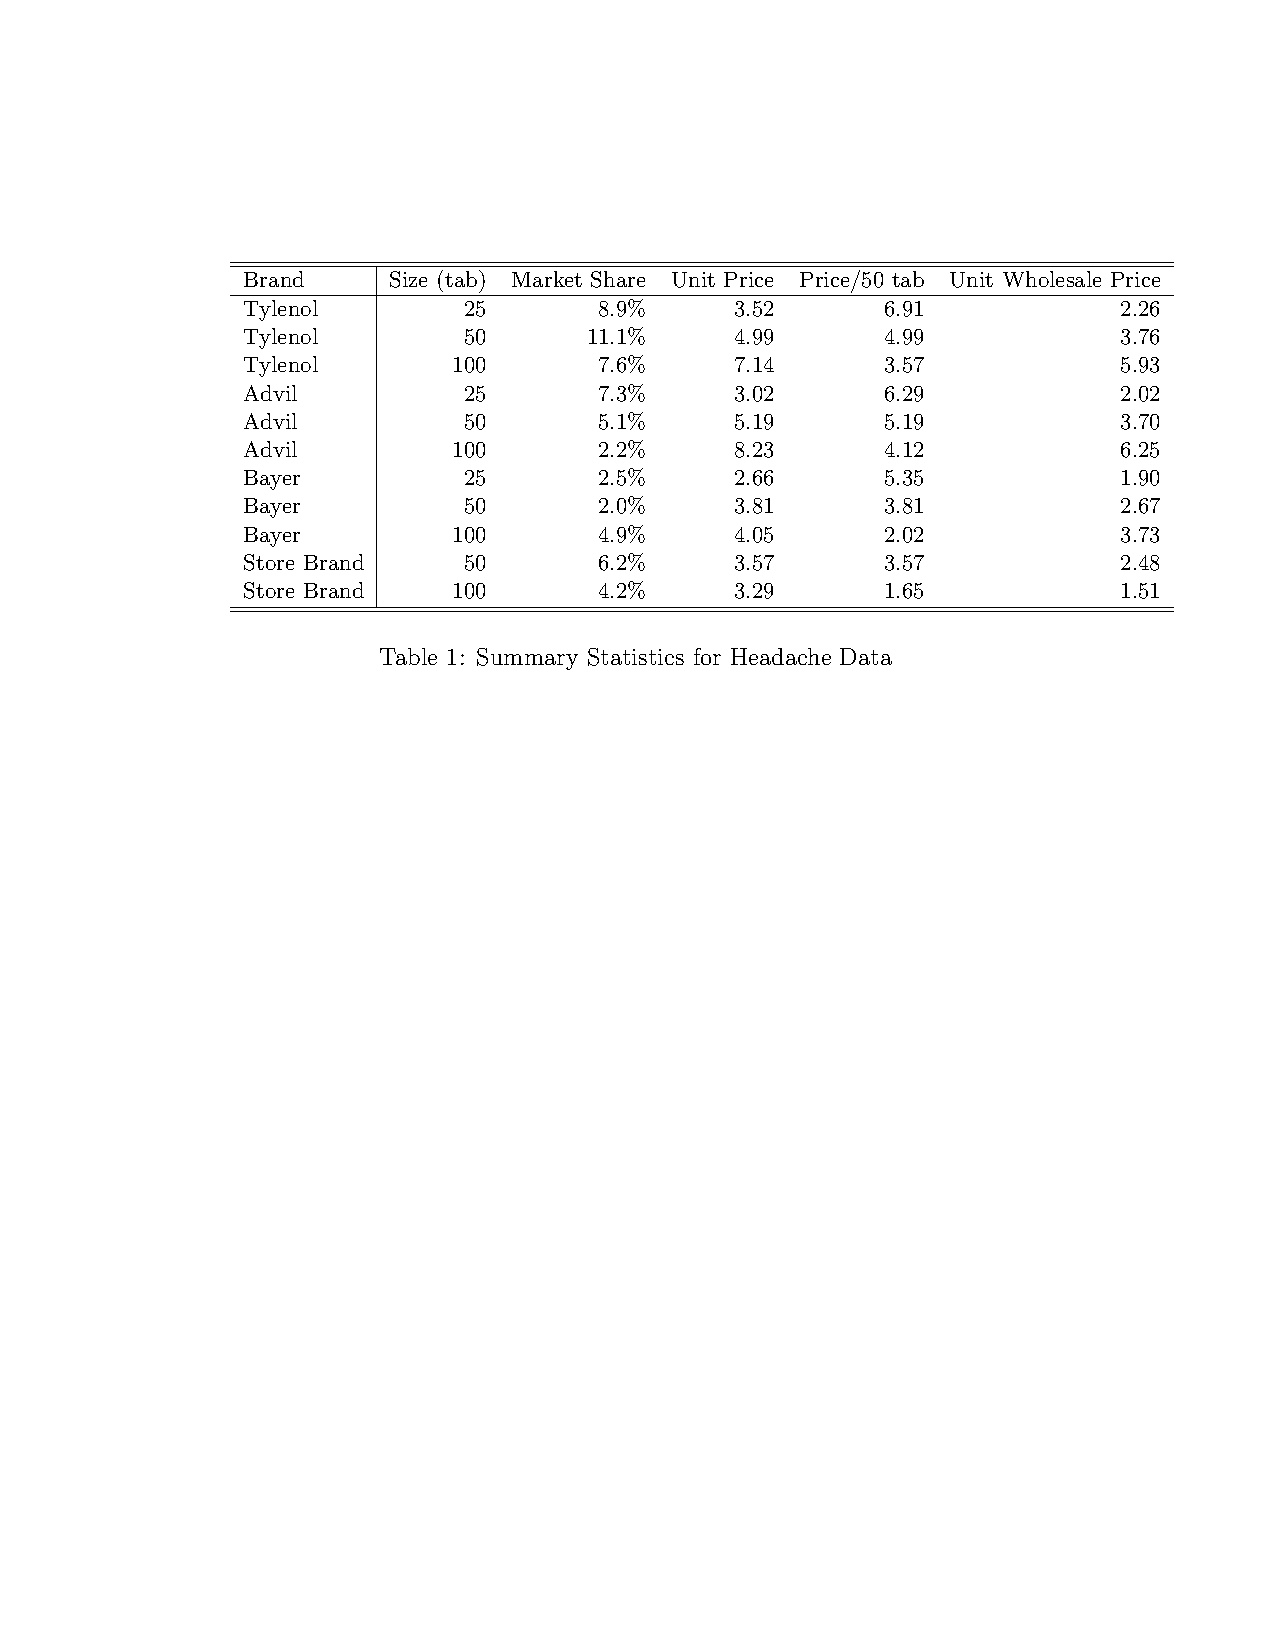
\includegraphics{./resources/table1.pdf}
\subsection*{Linear Part: Logit Estimator}
Hint: It is tricky to create your own sets of multiple fixed effects in MATLAB  use \texttt{dummyvar}. In R these are easier to construct. Recall that there are two ways to include FE (dummy variables and first difference).

You can report all of the following in one or two nicely organized tables.\\

For this setting assume that $\alpha_i = \alpha$ and $\beta_i = \beta$ (we have no random coefficients)
\begin{enumerate}
\item Estimate the mean utilities $\delta_{jt}$ using the inversion. Write the algebra, and store this in a variable \texttt{delta}.
\item Using OLS for  $\delta_{jt}$ with price and promotion as product characteristics.
\item Same as above. Add brand FE. Write down the equation for $\Delta \xi_{jt}$ the new structural error.
\item Same as above. Add brand $\times$ store FE.  Write down the equation for $\Delta \xi_{jt}$ the new structural error.
\item Estimate (2)-(4) using IV and the COST instruments only.
\item Estimate (2)-(4) using IV and the Hausman instruments only (average price in other markets).
\item Estimate (2)-(4) using IV and the both sets of instruments plus the average characteristics of other products in the same market (BLP) instruments.
\item Write the analytic formula for the Logit model and compute the mean own price elasticities by brand in the final week. Either a graph or a table. Do the estimates make sense? What is true about the ``premium'' brands?
\item How do the first-stage F-statistics look for each possible set of instruments?
\item Take All Quadratic interactions of all instruments. Project these interactions onto the principal components. Show how including additional principal components changes your estimates. How many principal components is enough?
\end{enumerate}

\subsection*{Random Coefficients Logit Estimator (Extra Credit)} 
\textit{I provide code for this on}  \url{http://www.github.com/chrisconlon/blp-demand/}, \textit{linked from my webpage. The code is in \texttt{MATLAB} but easy to use (hopefully).} \\

\noindent Now we incorporate the following two random coefficients:
\begin{itemize}
\item $\alpha_i = \alpha + \pi y_i$ where $y_i$ is income. (make sure you merge this in correctly in the previous part).
\item $\beta_{i}^B \sim N(\beta^b,\sigma_b)$ a random coefficient on a new variable \texttt{branded} which $=1$ for branded products and $=0$ for generic or store-brand products.
\end{itemize}
You will want to expand the set of Hausman instruments. Instead of using the average of the price of the same product in other stores during the same week, use all of the prices of the same product in other stores in the same week (or at least 30 of them).\\

\noindent Answer the following:
\begin{enumerate}
\item Do we need a random coefficients estimate a model with $\alpha_i$ but not $\beta_i$? Report these results for OLS and IV using all of the instruments and brand-dummies and promotion as your $x$ variables.
\item Now suppose we also allow for a random coefficient on $\beta_i^{B}$ the branded dummy in addition to the $\alpha_i$ parameter. I suggest using Gauss-Hermite quadrature rules (see \url{www.sparse-grids.de} for MATLAB program to generate these rules). Use brand-dummies and promotion as your $x$ variables. You will want to estimate $[\alpha, \pi, \sigma_b]$. The code should return the standard errors.
\item Again compute the average own price elasticities (make sure to write down the correct formula which allows for random coefficients). How do the own and cross price elasticities compare to the logit model? You can show this just for a single store in a single week.
\end{enumerate}
\textit{My code makes the distinction between the nonlinear parameters (which have random coefficients) which it calls \texttt{x2} and the linear part of utility which it calls \texttt{x1}. The linear part of utility should NOT include prices, you will need a separate variable \texttt{price}. The instruments \texttt{z} only need to include the excluded instruments not the other regressors. The program always returns the nonlinear parameters first, followed by  \texttt{price} and then the rest of \texttt{x1}. The Nevo Practicioner's Guide explains the linear/nonlinear parameter distinction.} 

\end{document}


